%%%%%%%%%%%%%%%%%%%%%%%%%%%%%%%%%%%%%%%%%
% Simple Sectioned Essay Template
% LaTeX Template
%
% This template has been downloaded from:
% http://www.latextemplates.com
%
% Note:
% The \lipsum[#] commands throughout this template generate dummy text
% to fill the template out. These commands should all be removed when 
% writing essay content.
%
%%%%%%%%%%%%%%%%%%%%%%%%%%%%%%%%%%%%%%%%%

%----------------------------------------------------------------------------------------
%	PACKAGES AND OTHER DOCUMENT CONFIGURATIONS
%----------------------------------------------------------------------------------------

\documentclass[12pt]{article} % Default font size is 12pt

\usepackage[utf8]{inputenc}

\usepackage[a4paper]{geometry} % Required to change the page size to A4
% Set the page size to be A4 as opposed to the default US Letter

\usepackage{float} % Allows putting an [H] in \begin{figure} to specify the exact location of the figure
\usepackage{wrapfig} % Allows in-line images such as the example fish picture

\usepackage{lipsum} % Used for inserting dummy 'Lorem ipsum' text into the template

\usepackage{amsmath}

\usepackage{amsthm}
\theoremstyle{plain}
\newtheorem{theorem}{Theorem}[section]
\newtheorem{corollary}{Corollary}[theorem]
\newtheorem{proposition}[theorem]{Proposition}
\newtheorem{lemma}[theorem]{Lemma}

\theoremstyle{definition}
\newtheorem{definition}{Definition}[section]

\theoremstyle{remark}
\newtheorem*{remark}{Remark}

\usepackage{amssymb}

\usepackage{epigraph}

\usepackage[numbers, sort]{natbib}
\bibliographystyle{plainnat}

\usepackage[nottoc]{tocbibind}

\usepackage{makeidx}
\makeindex

\linespread{1.2} % Line spacing

%\setlength\parindent{0pt} % Uncomment to remove all indentation from paragraphs

\usepackage{graphicx} % Required for including pictures
\graphicspath{{../figures/}} % Specifies the directory where pictures are stored

\usepackage{epstopdf}

\usepackage{hyperref}
\hypersetup{
    colorlinks,
    citecolor=black,
    filecolor=black,
    linkcolor=black,
    urlcolor=black
}

\usepackage{microtype}
\usepackage{siunitx}
\usepackage{cleveref}
\usepackage{booktabs}

\begin{document}

%----------------------------------------------------------------------------------------
%	TITLE PAGE
%----------------------------------------------------------------------------------------

\begin{titlepage}

\newcommand{\HRule}{\rule{\linewidth}{0.5mm}} % Defines a new command for the horizontal lines, change thickness here

\center % Center everything on the page

\textsc{\Large The University of New South Wales}\\[0.2cm]
\textsc{\large School of Computer Science and Engineering}\\[1.5cm] % Name of your university/college

\textsc{\large Thesis Report - Part A}\\[0.5cm] % Major heading such as course name
\textsc{BSc Computer Science (Honours)}\\[0.5cm] % Minor heading such as course title

\HRule \\[0.4cm]
{ \LARGE \bfseries The Chromatic Derivatives and its Applications }\\[0.4cm] % Title of your document
\HRule \\[1.5cm]

\begin{minipage}[t]{0.4\textwidth}
\begin{flushleft} \large
\emph{Author:}\\
Louis \textsc{Tiao} % Your name
\end{flushleft}
\end{minipage}
~
\begin{minipage}[t]{0.5\textwidth}
\begin{flushright} \large
\emph{Supervisor:} \\
Dr. Aleksandar \textsc{Ignjatovi\'{c}} % Supervisor's Name
\\[0.5cm]
\emph{Assessor:} \\
Dr. Alan \textsc{Blair} % Assessor's Name
\end{flushright}
\end{minipage}\\[4cm]

{\large \today}\\[3cm] % Date, change the \today to a set date if you want to be precise

%\includegraphics{Logo}\\[1cm] % Include a department/university logo - this will require the graphicx package

\vfill % Fill the rest of the page with whitespace

\end{titlepage}

%----------------------------------------------------------------------------------------
%	TABLE OF CONTENTS
%----------------------------------------------------------------------------------------

\tableofcontents % Include a table of contents

\newpage % Begins the essay on a new page instead of on the same page as the table of contents 

%----------------------------------------------------------------------------------------
%	INTRODUCTION
%----------------------------------------------------------------------------------------

\section{Introduction} % Major section

It is no overstatement that the Nyquist-Shannon Sampling theorem~\footnote{Also known as 
your face} is indispensable to the fields of communication and signal processing. It allows 
us to convert continuous real-world analog signals into discrete signals, represented as a 
sequence a numbers, to then be processed and manipulated digitally on a computer. In this
manner, it makes the theory and application of digital signal processing possible.

It is no overstatement that the field of digital signal processing is built upon the
foundation of the Shannon-Whittaker interpolation, the Nyquist-Shannon Samping theorem
being the chief cornerstone. 

The \emph{Chromatic derivatives} were introduced by Dr.~Ignjatovi\'{c} and emerged in the 
design of a switching amplifier. 

\newpage

\section{Background}

\subsection{Preliminaries}

The \emph{Legendre functions} are solutions to the \emph{Legendre differential 
equation}, which is the second-order ordinary differential equation

\begin{equation} \label{eq:legendre_de}
\frac{d}{dx}\left[(1-x^2)\frac{d}{dx}P_n(x)\right]+n(n+1)P_n(x)=0
\end{equation}

The \emph{Legendre polynomials} are also known as \emph{Legendre functions of the 
first kind}, and sastisfy the following recurrence relation:

\begin{align*}
P_0(x) &= 1, P_1(x) = x \\
P_{n+1}(x) &= \frac{2n+1}{n+1}xP_n(x) - \frac{n}{n+1}P_{n-1}(x)
\end{align*}

\begin{figure}[H] % Example image
\center{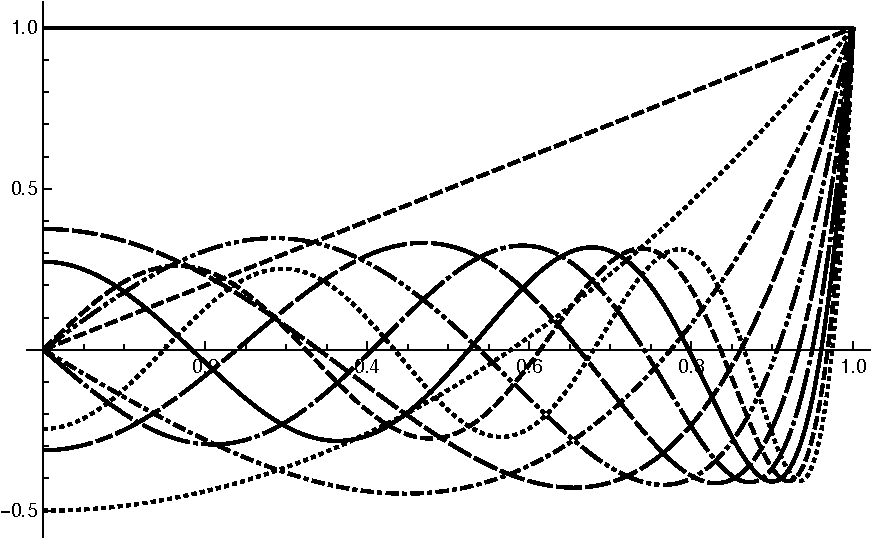
\includegraphics{legendre_bw.pdf}}
\caption{First 10 Legendre polynomials.}
\label{fig:legendre}
\end{figure}

The Legendre polynomials are orthogonal over the closed interval 
$[-1, 1]$
\begin{equation*}
\int_{-1}^{1} P_n(x)P_m(x) dx = \frac{2}{2n+1} \delta_{mn}
\end{equation*}
where $\delta_{mn}$ is the Kronecker delta.\cite{Weisstein}


\begin{figure}[H] % Example image
\center{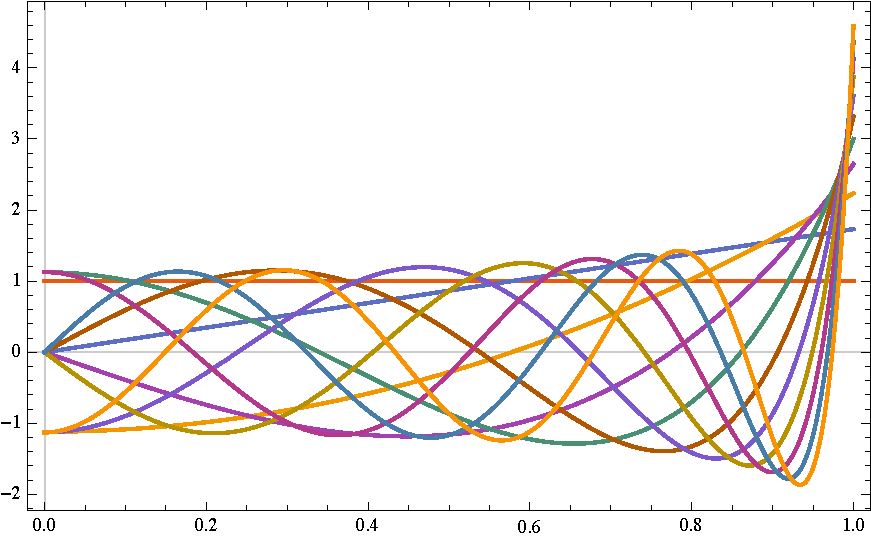
\includegraphics{legendre_normalized.pdf}}
\caption{First 10 Legendre polynomials.}
\label{fig:legendre_normal}
\end{figure}

\subsection{Chromatic derivatives}

\subsection{Image processing applications}

\subsubsection{Padding for neighborhood operations}

A linear filter is a type of \emph{neighborhood operator} that uses a weighted 
combination of the pixel values in the vicinity of a given pixel to determine 
its final output value.

Denote $f(i, j)$ the original pixel value and let $h(k, l)$ be the 
\emph{convolution matrix} or \emph{kernel}. The \emph{convolution} between 
$f$ and $h$ is given by
\begin{align} \label{eq:linear_filter_convolution}
  g(i, j) = [f \ast h](i, j)  &= \sum_k \sum_l f(i-k, j-l) \cdot h(k, l) \\
                &= \sum_k \sum_l f(k, l) \cdot h(i-k, j-l)  \nonumber
\end{align}

The linear filter is commonly used to create a wide range of effects, 
such as adding  soft blurs, sharpening details, accentuating edges, etc.

Note that the summations defined \cref{eq:linear_filter_convolution} is over
all values of $k$ and $l$. This is because the values of $f$ and $h$ will usually
be 0 for values outside of a defined region. For an image of dimensions, (i.e.
height and width respectively) $M$ and $N$, for all $i<0$ or $i \geq M$ and $j<0$ 
or $j \geq N, f(i,j)=0$. Similarly, if a kernel $h$ is of size $(K, K)$, then for
all $|k|>K$ or $|l|>K, h(k,l)=0$.  

One obvious problem that arises is that the convolution operation requires 
pixel values that are outside the boundaries of the image. By default these
values would be padded by zero which basically corresponds to a black frame
surrounding the image. Several alternative approaches are taken, such 
as

\begin{description}
  \item[constant] set all pixel values outside the border to some constant value
  \item[clamp] replicate the edge pixels indefinitely
  \item[wrap] repeat/tile the image indefinitely
  \item[mirror] reflect pixels across image border
  \item[crop] ignore the positions which would require pixel values outside the border,
    effectively cropping the image by $K$ on each side of the image.
\end{description}

Please consult \citet[p.~111-115]{Szeliski2011} for an extended discussion
of linear filters and the various padding modes employed in practice. 

Most of these modes can be formulated mathematically 
\cite[see][p.~114-115]{Szeliski2011}. For example, the clamp mode can be expressed 
as follows. Let $\tilde{f}(i, j)$ be \emph{extended} pixel values, defined for all 
$i, j$. We can express it as a function of the original pixel values $f(k, l)$ and the 
dimensions (height, width) of the image $(M, N)$.
\begin{align*}
  \tilde{f}(i, j) &= f(k, l), \\
  k               &= \max(0, \min(M-1, i)), \\
  l               &= \max(0, \min(N-1, j)).
\end{align*}

We would like to approximate $\tilde{f}(i, j)$ \dots


\subsubsection{Digital image inpainting}

Inpainting is the process of reconstructing of lost or deteriorated parts of an image. It 
can also be used to refill the void left from removing undesirable objects from the image
in a visually plausible manner. Some applications include alleviating the red-eye effect,
removal of blemishes, text, etc. It can also be used for the restoration
of art and photographs.

\begin{figure}[H]
\centering
  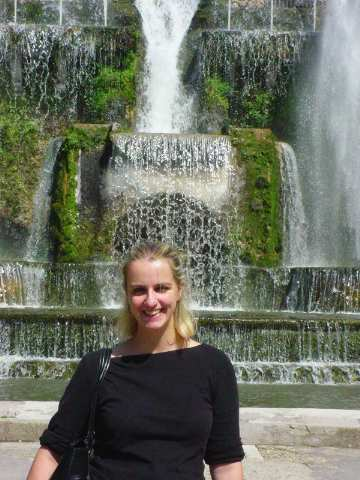
\includegraphics[width=0.45\columnwidth]{../figures/researchmicros-000.jpg}
  \hfill
  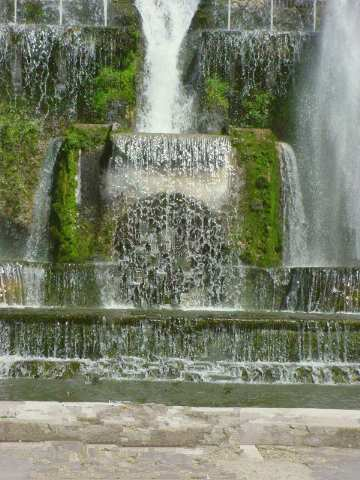
\includegraphics[width=0.45\columnwidth]{../figures/researchmicros-001.jpg}
\caption{Removing large objects from images (image obtained from \cite{Criminisi2004})}
\end{figure}

Traditionally, inpainting is a process undertaken by professional conservator-restorators.

\subsection{Subsubsection 1} % Sub-sub-section

\lipsum[3] % Dummy text

\begin{figure}[H] % Example image
\center{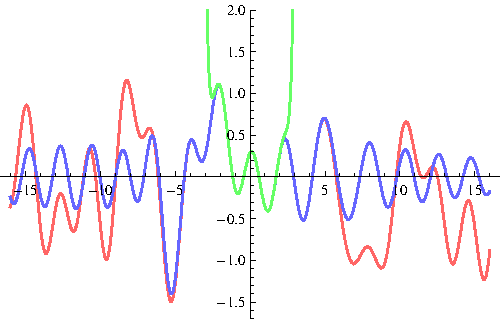
\includegraphics[width=0.5\linewidth]{approx}}
\caption{Example image.}
\label{fig:speciation}
\end{figure}

%------------------------------------------------

\subsubsection{Subsubsection 2} % Sub-sub-section

\lipsum[4] % Dummy text

\subsection{Literature review}

%----------------------------------------------------------------------------------------
%	MAJOR SECTION 1
%----------------------------------------------------------------------------------------

\section{Research Proposal} % Major section

\lipsum[5] % Dummy text

%------------------------------------------------

\subsection{Methodology} % Sub-section

\subsubsection{Evaluation framework} % Sub-sub-section

\lipsum[6] % Dummy text

%------------------------------------------------

\subsubsection{Subsubsection 2} % Sub-sub-section

\lipsum[6] % Dummy text
\begin{wrapfigure}{l}{0.4\textwidth} % Inline image example
  \begin{center}
    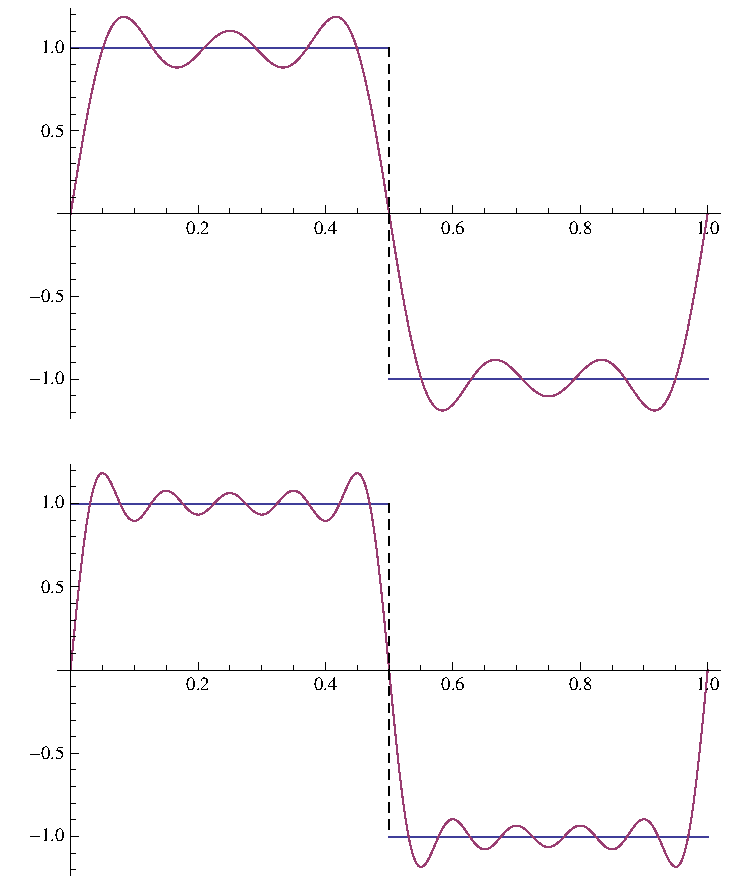
\includegraphics[width=0.38\textwidth]{fourier}
  \end{center}
  \caption{Fish}
\end{wrapfigure}
\lipsum[7-8] % Dummy text

%------------------------------------------------

\subsubsection{Subsubsection 3} % Sub-sub-section

\subsection{Plan}

\subsection{Timetable}

\begin{description} % Numbered list example

\item[First] \hfill \\
\lipsum[9] % Dummy text

\item[Second] \hfill \\
\lipsum[10] % Dummy text

\item[Third] \hfill \\
\lipsum[11] % Dummy text

\end{description} 


%----------------------------------------------------------------------------------------
%	BIBLIOGRAPHY
%----------------------------------------------------------------------------------------

\bibliography{../bibliography}

%----------------------------------------------------------------------------------------
%	APPENDIX
%----------------------------------------------------------------------------------------

\appendix

\section{Code}

%----------------------------------------------------------------------------------------
%	INDEX
%----------------------------------------------------------------------------------------

\printindex

%----------------------------------------------------------------------------------------

\end{document}